\documentclass[letterpaper,12pt]{article}
\usepackage[margin=2cm]{geometry}

\usepackage{graphicx}
\usepackage[colorlinks=true]{hyperref}

\newcommand{\panhline}{\begin{center}\rule{\textwidth}{1pt}\end{center}}

\title{\textbf{Safe Walk -- Gait Monitoring System\\\small (17S WSN Project)}}
\author{Emily Ruppel, Iljoo Baek, Mengwen He (Team 11)}

\begin{document}
\maketitle

\begin{figure}[!h]
	\centering
	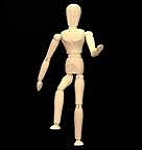
\includegraphics[width=3cm]{./imgs/marven.jpg}
\end{figure}

\panhline
\section{Contents}
\begin{itemize}
	\item \href{./Motivation/document.html}{Motivation}
	\item \href{./Introduction/document.html}{Introduction}
	\item \href{./Sensors/document.html}{Sensors}
	\item \href{./Communication/document.html}{Communication}
\end{itemize}

\panhline
\section{Resources}
\begin{itemize}
	\item \href{./PDFs/GaitMonitoring_Feb-24-17_v0.1.pdf}{Proposal PPT}
	\item \href{./PDFs/proposal_grp11.pdf}{Proposal}
\end{itemize}

\panhline
\section{Schedule}

\begin{figure}[!h]
	\centering
	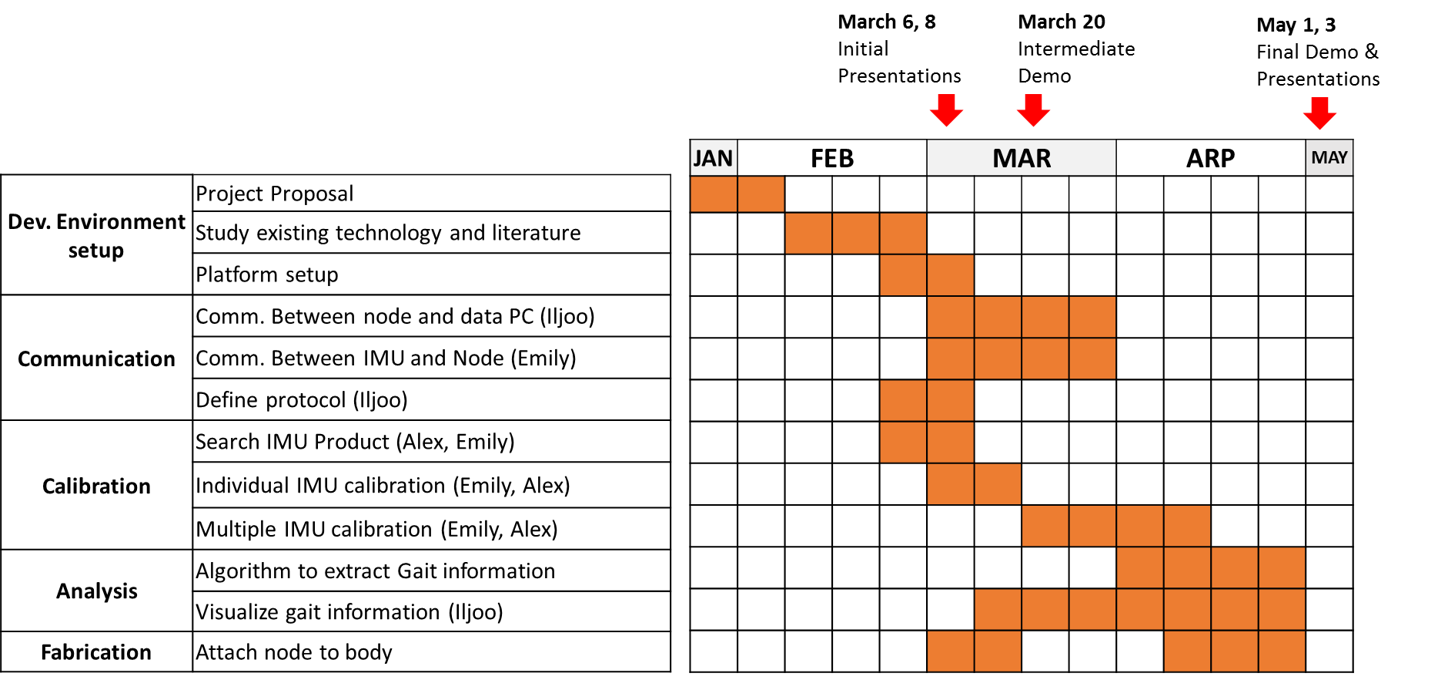
\includegraphics[width=15cm]{./imgs/schedule.png}
\end{figure}

\panhline
\section{Events}

\subsection{2017-03-03 Meeting}

\begin{itemize}
	\item Done
	\begin{itemize}
		\item Finished the proposal documentation
		\item Built a website on GitHub
		\item IMU Sensor:
		\begin{itemize}
			\item Got 4 Razor IMU sensors
			\item Tested it with ROS, and checked its output
			\item Decided to transmit binary data stream via RF and serial port
		\end{itemize}
	\end{itemize}
	\item ToDO
	\begin{itemize}
		\item Develop an interface between serial port and ROS
		\item Modify the IMU firmware to output raw + calculated data
		\item Build the communiation from IMU to Firefly
		\item Build the communiation from Firefly to PC
		\item Solve the time synchronization problem		
	\end{itemize}
\end{itemize}

\subsection{2017-03-04 Camera+IMU Development Based on ROS+RobotSDK}

\begin{figure}[!h]
	\centering
	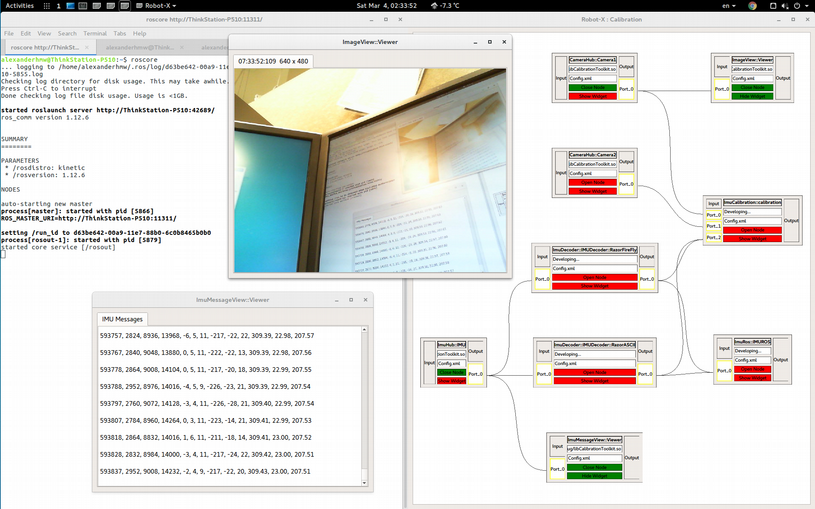
\includegraphics[width=20cm]{./imgs/cameraimu.png}
\end{figure}

\panhline



\end{document}